%        File: siip.tex
%     Created: Mon Feb 27 08:00 AM 2017 C
% Last Change: Mon Feb 27 08:00 AM 2017 C
%
\documentclass[11pt]{article}

%\usepackage[acronym,toc]{glossaries}
%\include{acros}
%\makeglossaries
\usepackage{fancyhdr}
\usepackage{pagecounting}
\usepackage[dvips]{color}
\usepackage{graphicx}
\usepackage{caption}
\usepackage{subcaption}
\usepackage{placeins}
\usepackage[hidelinks]{hyperref}
\usepackage{tabularx}

% Trying to bold PI names in the bib
\usepackage{xstring}
\def\FormatName#1{%
          \IfSubStr{#1}{Huff}{\textbf{#1}}{\IfSubStr{#1}{Neal Davis}{\textbf{#1}}{#1}}%
          }

          \usepackage[left=1in, right=1in, top=1in, bottom=1in]{geometry}
          \newcommand\bb[1]{\mbox{\em #1}}
          \def\baselinestretch{1.1}
          %\pagestyle{empty}
          \newcommand{\hsp}{\hspace*{\parindent}}
          \definecolor{gray}{rgb}{0.4,0.4,0.4}

          \newcommand{\authorname}{Kathryn~D.~Huff }
          \newcommand{\authoremail}{kdhuff@illinois.edu}
          \newcommand{\authorsite}{arfc.npre.illinois.edu}

          \begin{document}
          \title{Collaborative Open-Source Curriculum Development}
          \author{\textbf{PI: Kathryn Huff}\\%
                  kdhuff@illinois.edu\\
                  University of Illinois at Urbana--Champaign
                  \and
           \textbf{Co-PI: Neal Davis}\\
                  davis68@illinois.edu\\
                   University of Illinois at Urbana--Champaign
                  \and
           Paul Wilson\\
                  University of Wisconsin - Madison 
                  \and
          Steven Skutnik\\
                  University of Tennessee - Knoxville
                  \and
          Anthony Scopatz\\
                  University of South Carolina 
                  \and
          Jeremy Roberts\\
                  Kansas State University 
                  \and
          Robert Borrelli\\
                  University of Idaho at Idaho Falls
          }
          \maketitle

          \pagestyle{fancy}
          %\pagenumbering{gobble}
          %\fancyhead[location]{text}
          % Leave Left and Right Header empty.
          %\lhead{}
          %\rhead{}
          \lhead{\textcolor{gray}{SIIP Full Proposal}}
          \rhead{\textcolor{gray}{Collaborative Open-Source Curriculum Development}}
          %\rhead{\textcolor{gray}{\thepage/\totalpages{}}}
          \renewcommand{\headrulewidth}{0pt}
          \renewcommand{\footrulewidth}{0pt}
          %\fancyfoot[C]{\footnotesize \textcolor{gray}{\authorsite}}

          \section{Problem}
          At this very moment, professors at scores of institutions in the United States are 
          simultaneously preparing lessons on transposing a matrix.
          They are doing so largely without receiving feedback from one another 
          or directly building on one another's experience 
          \cite{green_building_2014}. In this way, 
          professors spend an enormous amount of time duplicating curriculum 
          development efforts already tackled by colleagues. What's worse is 
          that these efforts are rarely, if ever, reviewed by, shared with, or 
          extended upon by peers. We would never conduct research in such a 
          closed fashion -- why are we teaching this way?
          %Q:  If the process of lesson preparation is valuable in ordering one's thoughts,
          % doesn't an "on-tap" curriculum sap instructor effectiveness?
          
          Open-source software development suggests a possible collaborative solution.
          These communities have mastered the challenges of distributed expert collaboration, 
          dynamic peer review, and de-duplication of effort. In open-source 
          software development workflows, developers share code revisions in online repositories, 
          review one another's work in small chunks \cite{wilson_best_2014}, 
          and contribute back their own improvements to the main project.
          Thus open-source projects can focus concentration on particularly needed tasks
          even from diffuse effort.

          So why aren't professors sharing their lesson materials online, 
          collaborating on canonical lesson sets, diffing and merging similar 
          lessons, and reviewing one another's learning materials?
          Previous attempts at collaborative curriculum development have met with 
          challenges, including instructor inertia, an unclear process for collaboration,
          lack of a committed core team, differing visions, and particular institutional needs.
          %Q:  Why?  If you raise the question, we need at least a stab at an answer here.
          % I know for myself the fact that I work in triage is a major factor.
          \textbf{Our goal is to explore the possibility that curriculum development for 
          university courses can operate as well as open source software development 
          does.}
          
          Most notable among efforts toward collaborative curriculum 
          development is the Software Carpentry Foundation (a program
          which the PI and Co-PI have been quite involved with) 
          \cite{wilson_software_2014}.  Since 2011, the Software Carpentry program has taught 
          computational skills for scientists using a shared curriculum hosted 
          on GitHub. Hundreds of instructors across the planet use and remix 
          the lesson materials. Unfortunately, our experience showed that while these 
          instructors used and improved on the original material, they rarely 
          contributed their changes back to the master material. Thus, versions 
          of the original material tend to diverge rather than converge 
          \cite{wilson_software_2014,wilson_software_2014-1}.
          
          We expect a granular lesson plan---combining fine-grained lesson components
          with a clear dependency graph of prerequisite modules---to assist in 
          overcoming the challenges encountered by Software Carpentry and 
          others.

          \section{Proposed Solution}
          We propose a small-scale proof-of-concept for collaborative
          open-source curriculum development effort to improve the \emph{transfer of lessons 
          learned} between instructors of the same course (either at a single 
          university or among different campuses). This pilot collaboration 
          will provide a template which could be adopted for collaboration 
          among faculty teaching courses with an inherently larger scale (e.g. 
          introductory CS1 courses like CS101).

          \subsection{Collaboration Roles}
          Faculty in Nuclear Engineering from five institutions\footnote{
          Paul Wilson at (UW Madison), 
          Steven Skutnik (UT Knoxville), 
          Anthony Scopatz (University of South Carolina), 
          Jeremy Roberts (Kansas State University), 
          and Robert Borrelli (University of Idaho)
          } have agreed to be participants in 
          this prototyping effort. We all currently use 
          \href{https://github.com}{GitHub} as a platform to store, 
          revise, and collaborate on research, particularly source code. 
          Additionally, many have already begun to host their individual course 
          materials online as well, but to date these have so far been single-author 
          repositories (e.g. \cite{huff_npre412_2017}).
          % jar:  I'm not really sure what you mean by this last statement.  Are 
          %       some in the group already working with you on this type of course?

          The participants will collaborate on a master set of learning 
          modules for an upper-division course in nuclear engineering: 
          The Nuclear Fuel Cycle. In the near term, we will develop 
          fine-grained lessons and assessments which may be mixed and matched 
          to meet the learning objectives. The curriculum will be hosted on 
          GitHub, tested by all of us, and improved continually.
          
          The PI and external collaborators will contribute and develop lesson 
          material including lesson notes, in-class exercises, worked example 
          problems, assessments (homework, quiz, and test questions), project 
          assignment descriptions, media (images, movies), supporting material 
          references, etc. These collaborators will primarily rely on the 
          material they have developed for their own courses, but will need to 
          convert that material into the format of the collective resource 
          (format practicalities to be decided at the first workshop). Additionally, these 
          collaborators will be core maintainers of the repository and will 
          accordingly be responsible for conducting reviews of new material 
          pull requests.

          Prof.~Neal Davis, Co-PI of this proposal, has contemplated a 
          Collaborative Computational Curriculum for some time 
          \cite{davis_university_2016}. Since he 
          teaches large-scale computational curriculum at Illinois 
          he is an ideal person to potentially scale-up this work at Illinois in the 
          future. Additionally, he has the nuclear engineering background to 
          understand the context of this prototyping effort (the nuclear fuel 
          cycle). Prof.~Davis' role 
          in this effort will be to conduct \emph{action research}, observing 
          our process and teasing out potential avenues for future 
          extensions and applications of the process. 

          \subsection{Open-Source Workflow}
          Development of this proof-of-concept curriculum will be undertaken 
          similarly to an open-source software project. 
          In particular, this work will emulate features of open-source software development 
          that cultivate distributed collaboration. By convention in the open-source community, for 
          example, new code features are described in \emph{issues} or 
          \emph{tickets} and discussed before implementation. Small, atomic 
          changes are reviewed before they are merged into the 
          \emph{repository}. These discussions and incremental reviews nurture 
          communities of practice.

          In a typical open-source project, a main copy of the 
          repository (or main \emph{fork}) holds the 
          official instance of the software package. Individual developers each have their own 
          \emph{forks} where they can work on features and 
          bug fixes. When the developer makes changes that are ready for prime 
          time, they make a ``pull request'' to the main \emph{fork}. That 
          \emph{pull request} is 
          reviewed by their collaborators, and if successful it is eventually merged into the 
          main fork where it can be used by all. Figures 
          \ref{fig:sub1} and \ref{fig:sub2} show how this open-source software 
          development workflow can be adapted for lesson development.

          \begin{figure}
                  \centering
                  \begin{subfigure}{.4\textwidth}
                            \centering
                            \includegraphics[width=.8\linewidth]{git-flow}
          \caption{This process, known as \emph{Git Flow}, through which a new 
                          feature or bug fix enters a piece of open source 
                          software\cite{scopatz_effective_2015}.}
                                  \label{fig:sub1}
                  \end{subfigure}\hfill%
                  \begin{subfigure}{.4\textwidth}
                            \centering
                            \includegraphics[width=.8\linewidth]{siip-flow}
          \caption{This adaptation of Git Flow reimagines the process in the context of learning module development.}
                                  \label{fig:sub2}
                  \end{subfigure}
                  \label{fig:test}
          \end{figure}
          \FloatBarrier

\iffalse
          Doing code review at the end of the work isn't useful. What works is 
          incremental code review. This proposal suspects that the same is true 
          for curriculum review.  \cite{wilson_software_2014}.

          Education is an inherently distributed system, but this need not be a hindrance to collaboration.

          Scientists are more than happy to build upon one another's work, form 
          collaborations with others in their field. But, 
          when it comes to educating, where is the sharing of lessons learned 
          and collaboration? 
\fi

          \section{Timeline and Deliverables}
          Briefly, the timeline will be as follows:

          \begin{itemize}
                  \item \textbf{Jul 2017} Kick-Off Workshop
                  \item \textbf{Aug 2017 - June 2017} Curriculum development
                  \item \textbf{Aug 2017 - Dec 2017} NPRE 412 beta testing
                  \item \textbf{Jul 2018} Retrospective Workshop
          \end{itemize}

          \subsection{Timeline}
          The year will be bookended by two workshops, a kickoff workshop 
          and a retrospective workshop. In the intervening time, the curriculum 
          will be developed. Consistent 
          communication through GitHub's collaboration framework, a Slack 
          channel, an email listhost, a shared Google Drive folder, and monthly 
          Google Hangouts will drive this work.

          Additionally, in Fall 2017, any material developed through this 
          process in time for fall will be incorporated into NPRE 412, the 
          University of Illinois nuclear fuel cycle course taught by the PI, 
          Kathryn Huff. Similary, the external participating faculty will 
          experiment with incorporating these materials into their courses at 
          their home institutions. 


          Details of the workshops and interim efforts are given in the next 
          subsections.

          \subsection{Kick-Off Workshop}
          A two-day kick-off workshop hosted at the University of Illinois at 
          Urbana-Champaign will allow the 
          participants to brainstorm and discuss the scope of the project.
          Among other potential products, the workshop will deliver
          a sketch of the initial framework of the collaborative effort and
          a logistical coordination of responsibilities. These products will
          be published in an online GitHub repository 
          and associated website.

          Invited participants in the first workshop will include Illinois PI Huff 
          and Illinois Co-PI Davis, external collaborating professors Wilson, 
          Skutnik, Roberts, Scopatz, and Borrelli, and up to 6 Illinois professors 
          who may be interested in adapting and extending this work for their own 
          future courses.

          As indicated in Table \ref{tab:kickoff}, products to be developed in 
          the first workshop include learning 
          objectives\cite{bloom_bloom_1984}, a concept 
          map\cite{novak_concept_1990}, 
          an outline of fine-grained lesson modules, and a 
          directed acyclic graph describing dependencies among lessons (similar 
          to the one in Figure \ref{fig:rosalind}). Additionally, concrete logistics 
          for completion will be established, including individual curriculum 
          development assignments, and a repository structure for organizing 
          the lesson material. Additionally, practical decisions will be made 
          such as establishing guidelines for lesson acceptability as well as 
          agreeing on raw formats for lesson content (markdown vs. \LaTeX, 
          Jupyter vs MATLAB, etc.),  At this workshop, interest and 
          compatibility with frameworks like RELATE 
          \cite{kloeckner_relate_2017,kloeckner_relate_2017-1} and tools like 
          PrarieLearn \cite{west_prairielearn:_2015} will be considered.

\begin{figure}[ht!]
        \begin{center}
                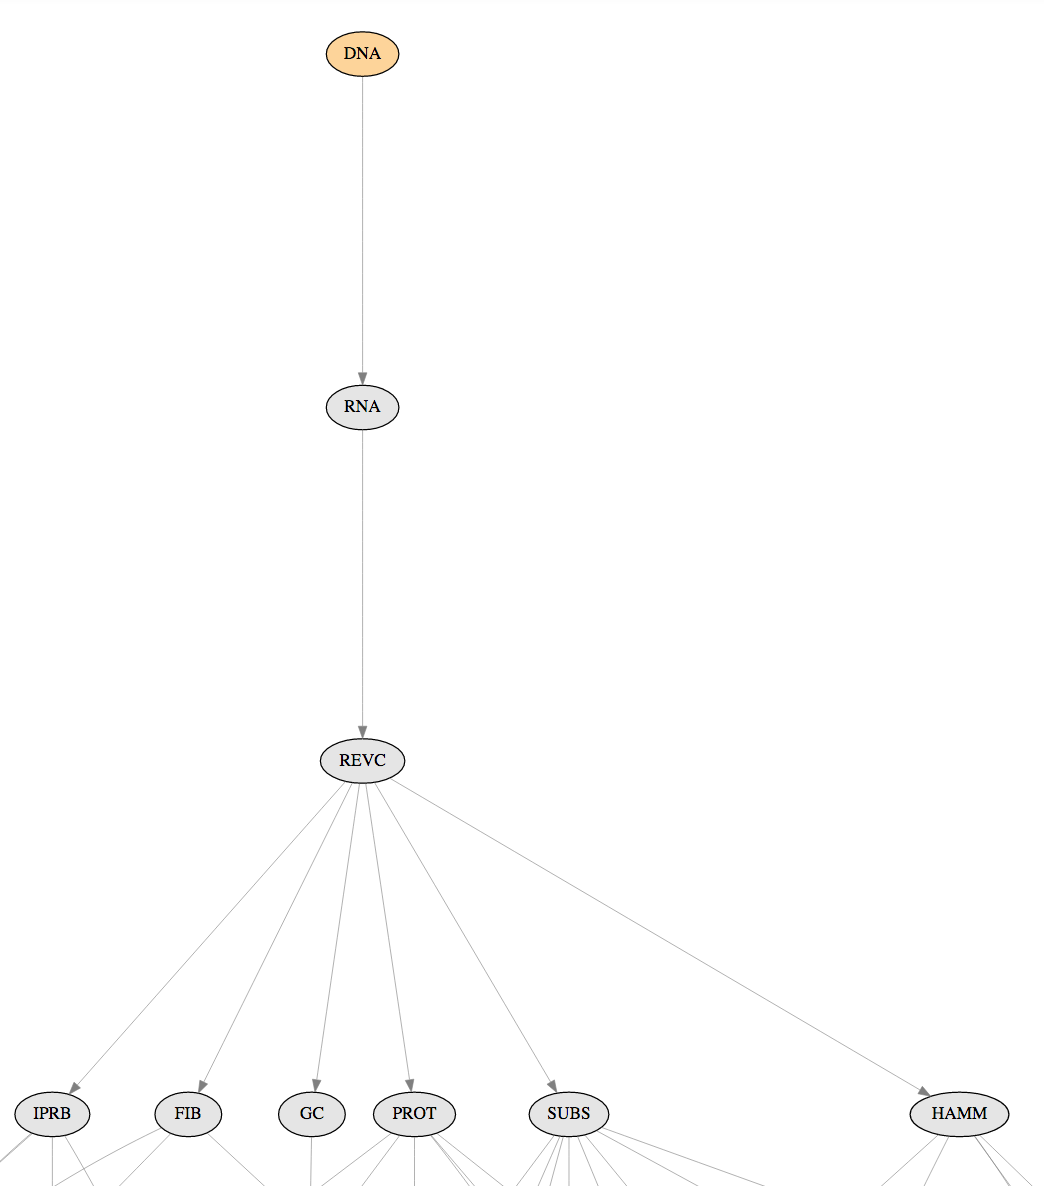
\includegraphics[height=0.5\textheight]{rosalind.png}
        \end{center}
        \caption{Rosalind.info, an educational bioinformatics resource, 
        organizes exercises based on their dependencies.}
        \label{fig:rosalind}
\end{figure}
          
          \begin{table}[h!]
                  \centering
          \begin{tabularx}{\textwidth}{r|l|l|X}
                                  \multicolumn{4}{c}{\textbf{Day 1}}\\
                                  \hline
                          \textbf{Time}& \textbf{Activity}& \textbf{Lead}& \textbf{Deliverable}\\
                                  \hline
8:00& Welcome and Breakfast& Huff \& Davis& \\
9:00& Vision Lightning Talk& Wilson& Idea Collection\\
9:15& Vision Lightning Talk& Skutnik& \\
9:30& Vision Lightning Talk& Scopatz& \\
9:45& Vision Lightning Talk& Roberts& \\
10:00& Vision Lightning Talk& Borrelli& \\
10:15& Vision Lightning Talk& Huff& \\
10:30& Break&&  \\
10:45& Concept Mapping Exercise& All& Curriculum Concept Map\\
12:00& Lunch& All& \\
13:00& Brainstorm Learning Objectives& All& Learning Objectives List\\
15:00& Break&&  \\
15:15& Refine Lesson Topics& All& Lesson Topics List\\
16:00& Discussion of Formats for Content& All&  \\
17:00& Break&&  \\
19:00& Dinner&&  \\
\hline
                                  \multicolumn{4}{c}{}\\
                                  \multicolumn{4}{c}{\textbf{Day 2}}\\
                                  \hline
                          \textbf{Time}& \textbf{Activity}& \textbf{Lead}& \textbf{Deliverable}\\
                                  \hline
8:00& Review and Breakfast& Huff \& Davis& \\
9:00& Lesson Dependency Exercise& All& Lesson Dependency Graph\\
10:30& Break&&  \\
10:45& Lesson Dependency Exercise& All& \\
12:00& Lunch& All& \\
13:00& Repository Initialization&&  Template Workspace\\
14:00& Determination of Milestones& All& Work Plan\\
15:00& Break&&  \\
15:15& Assigment of Responsibilities& All&  \\
16:00& Review and Wrap-up& All&  \\
17:00& Break&&  \\
19:00& Dinner&&  \\
\hline
                  \end{tabularx}
                  \caption{Preliminary schedule for the Kick-off Workshop}
                  \label{tab:kickoff}
          \end{table}


          \subsection{Interim Period}
          Between workshops, the PI and external collaborators will commence 
          work on developing 
          the fine-grained lesson modules. These lessons will be submitted by pull request to the main 
          repository and each lesson will include:
          \begin{itemize} 
                \item associated learning objectives (identified previously)
                \item content (e.g. speaking notes, presentation material, 
                      derivations, worked examples, active learning  
                      exercises, external readings, videos, images)
                \item learning assessments (e.g. project descriptions, exam questions) 
          \end{itemize} 

          Interactions will commence primarily via issues, pull requests, and 
          reviews on GitHub during this time. Meanwhile, monthly video 
          conferences will help to spur high-level conversation onward.
          Co-PI Davis will be invited to engage in these video conference as 
          part of action research toward the final 
          As progress is made, lessons learned will be recorded by all 
          participants in a draft instruction manual.
          % TODO: what of Sp18?

          \subsection{Retrospective Workshop}
          A two-day retrospective workshop (\$15K) at Illinois will wrap up the 
          project. Discussion concerning the process will allow reflection as 
          well as a collection of lessons learned.
          Experiences live testing the developed course material (for example 
          in NPRE412 at Illinois in Fall 2017) will be shared and suggested 
          improvements will be captured as feature requests on GitHub.  
          The lessons learned from the year-long process will be captured in a 
          template GitHub repository and in a collaboration instruction manual in 
          website form. 
          % Started a sentence with ``Futu...''  Maybe you had a thought to complete?
          
          With these resources, other groups of faculty seeking to collaborate 
          in a similar way can simply fork the template repository and follow 
          the instructions on the website to begin the process of developing 
          their domain curriculum.

          Invited participants in the retrospective workshop will include:

          \begin{itemize}
                  \item Illinois PI Huff and Illinois Co-PI Davis
                  \item external collaborating Professors Wilson, Roberts, 
                          Skutnik, and Scopatz
                  \item up to 6 Illinois professors interested in extending this 
                          work in the future for their own courses.
          \end{itemize}


          \section{Potential Impact}
          This work will have immediate student and faculty outcomes at all of 
          the six universities where faculty are participating
          (Illinois, UW Madison, UT Knoxville, the University of South Carolina, 
          Kansas State University, and the University of Idaho). 
          It will 
          additionally have long term student and faculty outcomes at Illinois. 
          Beyond this, it may have institutional outcomes at Illinois. 
          
          This work will provide an important proof of concept for groups of 
          instructors willing to collaborate on open source curriculum for:
          \begin{itemize}
                  \item core courses with many sections in a single university
                  \item niche courses taught by a select group of professors across 
          universities
                  \item fundamental courses in small fields (e.g. nuclear engineering)
          \end{itemize}

          \paragraph{Student Outcomes}
          Students enrolled in NPRE412 at Illinois and peer courses at partner 
          institutions (USC, UT---Knoxville, Kansas State University, the 
          University of Idaho, and UW---Madison) will have an improved 
          experience. Their 
          curriculum will be bolstered by the comprehensive concept maps 
          underlying their coursework\cite{novak_concept_1990}, as well as exercises 
          and assessment tools reviewed and improved by expert professors at 
          peer institutions. 

          \paragraph{Illinois Faculty Outcomes}
          The effort of developing curriculum in this way may be labor 
          intensive initially. However, if the experience is similar to that of 
          open-source software teams, the required maintenance effort will decrease 
          substantially as lessons approach maturity. Minor improvements and updates
          to the curriculum contributed by colleagues will be effectively `free'
          in the long term. 

          \paragraph{Illinois Institutional Outcomes} Openness and collaboration 
          both increase visibility. The leadership of Illinois College of 
          Engineering faculty in this effort, if successful, will be exemplary 
          of the forward-thinking nature of the college and the university at 
          large. Furthermore, extensions to this work may be competitive for  
          support from educational grant-making agencies such as the National 
          Science Foundation and even private foundations such as Moore and 
          Sloan. 
          % TODO may want a citation on the first sentence of the preceding re increased visibility

          \paragraph{External Outcomes} Of perhaps most relevance in the
          context of this work is the potential external impact. This effort
          should spawn an instruction-centric community of practice among
          colleagues previously primarily connected by research 
          in their specific technical subdomain. 
          The participating professors at Illinois, UW Madison, UT Knoxville, 
          the University of South Carolina, Kansas State University, and the 
          University of Idaho teach similar courses at their home institutions 
          in part because their research is in similar subfields. In research, 
          it's obvious that many of us might collaborate, and this effort will 
          nurture the same kind of collaboration within our teaching. This is 
          very fitting with the vision behind SIIP -- this kind of collaboration 
          accross institutions within a scientific subfield is essential to 
          ``teaching like we do research.'' 

          \section{Budget}
          The first workshop will be hosted at the Allerton Retreat Center, 
          where a small meeting room will be reserved. Visiting 
          invited workshop participants will be flown to Urbana-Champaign and 
          lodged at the Illini Union Hotel. Table \ref{tab:budget} provides 
          details related to the expenses for these workshops.

\begin{table}[h!]
        \begin{tabularx}{\textwidth}{|X|c|c|c|c|c|}
        \hline
        \textbf{Event} & \textbf{Item} & \textbf{Cost} & \textbf{Units} & \textbf{\$} & \textbf{Notes}\\ 
        \hline
Kick-off&Meeting Room&744&2&1488&Allerton, all day package\\
Workshop     &Projector      &200    &2      &400   &Allerton\\
        &Lodging        &130    &12     &1560   &Allerton guest rooms\\
        &Flights        &800    &6      &4800   &Estimated\\
        &Taxi           &20     &12     &240    &\\
        &Incidentals    &100    &6      &600    &\\
        &Dinner         &30     &24     &720    &In Champaign-Urbana\\
\hline
Retrospective&Meeting Room   &50     &2      &100    &Illini Union\\
Workshop     &Projector      &300    &2      &600   &Illini Union\\
        &Lodging        &150    &12     &1800   &Illini Union Hotel\\
        &Flights        &800    &6      &4800   &Estimated\\
        &Taxi           &20     &12     &240    &\\
        &Incidentals    &100    &6      &600    &\\
        &Continental breakfast  &8.5    &24     &204    &University Catering\\
        &Coffee Service &32.5   &4      &130    &\\
        &Lunch          &15    &24     &360    &University Catering\\
        &Dinner         &30     &24     &720    &In Champaign-Urbana\\
\hline
Co-Pi	&Week Summer Salary&	$1666.\bar{66}$	&3	&5000	&Action Research\\
	&Fringe Benefits	&$741.\bar{66}$	&3	&2225	&44.5\%\\
        \hline
        &\textbf{Total}&&&\textbf{29947}&\\
        \hline
\end{tabularx}
\caption{The majority of expenses will support travel for visitors and workshop 
necessities. Additionally, summer support for Prof. Davis will allow time for 
        preparation of document summarizing lessons learned from his action 
        research.}
\label{tab:budget}
\end{table}



          \section{Departmental Support}
          The Department of Nuclear, Plasma, and Radiological Engineering will 
          support this work in kind with release time for Kathryn Huff through 
          her Start-Up funds.  Additionally, NPRE will support workshop activities 
          with administrative effort and by providing space. Finally, 
          collaborating external participants will contribute in kind with 
          summer time hours.


          \bibliographystyle{katyunsrt}
          \bibliography{2017-siip}


          \end{document}


